\documentclass[12pt, twoside]{article}
\usepackage[letterpaper, margin=1in, headsep=0.2in]{geometry}
\setlength{\headheight}{0.6in}
%\usepackage[english]{babel}
\usepackage[utf8]{inputenc}
\usepackage{microtype}
\usepackage{amsmath}
\usepackage{amssymb}
%\usepackage{amsfonts}
\usepackage{siunitx} %units in math. eg 20\milli\meter
\usepackage{yhmath} % for arcs, overparenth command
\usepackage{tikz} %graphics
\usetikzlibrary{quotes, angles}
\usepackage{graphicx} %consider setting \graphicspath{{images/}}
\usepackage{parskip} %no paragraph indent
\usepackage{enumitem}
\usepackage{multicol}
\usepackage{venndiagram}

\usepackage{fancyhdr}
\pagestyle{fancy}
\fancyhf{}
\renewcommand{\headrulewidth}{0pt} % disable the underline of the header
\raggedbottom
\hfuzz=2mm %suppresses overfull box warnings

\usepackage{hyperref}

\fancyhead[LE]{\thepage}
\fancyhead[RO]{\thepage \\ Name: \hspace{4cm} \,\\}
\fancyhead[LO]{BECA / Dr. Huson / Geometry\\*  Unit 1: Segments, length, and area\\* 28 Sept 2022}

\begin{document}

\subsubsection*{1.11 Pretest review: Length and area}
\emph{Show units if given. Show calculation as an equation, starting with a capitalized variable.}
\begin{enumerate}
  \subsubsection*{Line segments, length, number lines}
  \item Given isosceles $\triangle CAT$ with $\overline{CA} \cong \overline{AT}$. On the diagram mark the congruent line segments with tick marks.
\begin{center}
  \begin{tikzpicture}[scale=0.8]
    \draw[thick] (0,0)node[below left]{$C$}--
      (4,0) node[below]{$A$}--
      (65:3.7) node[above]{$T$}--cycle;
  \end{tikzpicture}
  \end{center} \bigskip

\item Points $R=-9$ and $S=33$ are shown below. Find ${RS}$. \par \smallskip
  \begin{tikzpicture}[scale=0.22]
    \draw[<->] (-12,0)--(42,0);
    \foreach \x in {-10, -5,...,40}
      \draw[shift={(\x,0)}] (0pt,-16pt)--(0pt,16pt)node[below=5pt]{$\x$};
    \draw[fill] (-9,0) circle [radius=0.2] node[above]{$R(-9)$};
    \draw[fill] (33,0) circle [radius=0.2] node[above]{$S(33)$};
  \end{tikzpicture} \vspace{1.5cm}

\item Mark and label irrational number $\pi = 3.14159265358...$ on the number line below.\par \bigskip
\begin{tikzpicture}[scale=3]
  \draw[->] (0,0)--(5.1,0);
  \foreach \x in {0, 0.1,...,5.0}
    \draw[shift={(\x,0)}] (0pt,-1pt)--(0pt,1pt);
  \foreach \x in {0, 0.5,...,5.0}
    \draw[shift={(\x,0)}] (0pt,-3pt)--(0pt,3pt)node[below=20pt]{$\x$};
\end{tikzpicture}
        
\item Given $\overline{DEF}$, $DE=5 \frac{3}{4}$, and $EF=8 \frac{1}{2}$. Find ${DF}$ as a mixed fraction. \par \bigskip
  \begin{tikzpicture}
    \draw[thick] (0,0)--(8,0);
    \draw[fill] (0,0) circle [radius=0.05] node[below]{$D$};
    \draw[fill] (3,0) circle [radius=0.05] node[below]{$E$};
    \draw[fill] (8,0) circle [radius=0.05] node[below]{$F$};
  \end{tikzpicture}  \vspace{1.5cm}

  \item Measure and mark the lengths of the sides of the rectangle in centimeters. Find its perimeter. \par \medskip
  \begin{tikzpicture}
    \draw [thick] (0,0) rectangle (8,2);
  \end{tikzpicture}

\newpage
\subsubsection*{Perimeter and area}

\item The rectangle $ABCD$ with dimensions $AB=10$ inches, $BC=7$ in.
\begin{multicols}{2}
  \begin{flushleft}
  \begin{tikzpicture}
    \draw[thick] (0,0)--(4,0)--(4,3)--(0,3)--cycle;
    \draw[fill] (0,0) circle [radius=0.05] node[left]{$A$};
    \draw[fill] (4,0) circle [radius=0.05] node[right]{$B$};
    \draw[fill] (4,3) circle [radius=0.05] node[right]{$C$};
    \draw[fill] (0,3) circle [radius=0.05] node[left]{$D$};
    \node at (4.5, 1.5){7};
    \node at (2, -0.5){10};
  \end{tikzpicture}
  \end{flushleft}
  \begin{enumerate}
    \item Find the area of the rectangle. \vspace{1cm}
    \item Find its perimeter.
  \end{enumerate}
  \end{multicols}

\item The side $\overline{AB}$ of triangle $ABC$ is extended and an altitude to the vertex $C$ is drawn, as shown below. The triangle's height is $h=7.25$ and its base measures $AB=12.4$. Find the area of the triangle. \par \medskip
\begin{tikzpicture}[scale=0.8]
  \draw[thick]
    (0,0)node[below]{$A$}--
    (6,0)node[below]{$B$}--
    (7,4)node[above]{$C$} --cycle;
  \draw[dashed] (7,0)--(7,4);
  \draw[dashed, ->] (6,0)--(7.5,0);
  \draw (7,0)++(-0.3,0)--++(0,0.3)--+(0.3,0);
  \node at (7,2.2)[right]{$h=7.25$};
  \node at (3,0)[below]{$12.4$};
\end{tikzpicture}
  
\item Find the area of the compound rectangular shape. Use area formulas for full credit.
  \begin{flushleft}
  \begin{tikzpicture}[step=0.5]
    \draw[help lines] (0,0) grid (5,2) (0,2) grid (3,6);
    \draw[thick] (0,0)--(5,0)--(5,2)--(3,2)--(3,6)--(0,6)--cycle;
    \node at (5.5, 1){4};
    \node at (4, 2.5){4};
    \node at (2.5, -0.5){10};
    \node at (-0.5, 3){12};
  \end{tikzpicture}
  \end{flushleft}

\newpage
\item Given the circle $A$ with radius $r=3$. Leave exact answers, in terms of $\pi$.
  \begin{multicols}{2}
    \begin{enumerate}
      \item Find the circumference of circle $A$. \vspace{1cm}
      \item Find the area of the circle.\vspace{2cm}
    \end{enumerate}
    \begin{flushright}
    \begin{tikzpicture}[scale=.9]
      \draw (0,0) circle [radius=3];
      \draw[fill] (0,0) circle [radius=0.05] node[below right]{$A$};
      \draw[thick, -{>[scale=1.5]}] (0,0)--(30:3);
      \node at (2,0.5){$r=3$};
      \clip (0,0) circle [radius=3];
        \draw[help lines] (-4,-4) grid (4,4);
    \end{tikzpicture}
  \end{flushright}
  \end{multicols}

\item Find the area of the parallelogram shown with a base $b=5$ and height $h=3$. \par \medskip
  \begin{tikzpicture}[scale=.635]
    \draw[help lines] (-1,-1) grid (9,6);
    \draw[thick, ->] (-1.2,0) -- (9.4,0) node[below right]{$x$};
    \draw[thick, ->] (0,-1.2)--(0,6.4) node[left]{$y$};
    \draw[<->, thick] (1.5,1)--(1.5,4);
    \draw[thick] (2,1)--(7,1)--(8,4)--(3,4)--cycle;
    \node at (4.5,1)[below]{$5$};
    \node at (1.5,2.5)[left]{$3$};
  \end{tikzpicture}

\item Find the area of shape $ABCDE$ below, a triangle on a rectangle. The altitude $h$ of the triangle is $3.20$ centimeters and the base $EC=5.5$ cm. The rectangle is 1 cm tall. (diagram not to scale) \par \medskip
  \begin{tikzpicture}[scale=1.25]
    \draw (2,0)--(7,0);
    \draw[thick] 
      (2,0)node[left]{$E$}--
      (2,-1)node[left]{$A$}--
      (7,-1)node[right]{$B$}--
      (7,0)node[right]{$C$}--
      (4,3)node[above]{$D$}--(2,0);
    \draw[dashed] (4,0)--(4,3);
    \draw (4,0)++(0.3,0)--++(0,0.3)--+(-0.3,0);
    \node at (4,1)[right]{$h=3.20$ cm};
    \node at (4.5,-1)[below]{$5.5$ cm};
    \node at (7,-0.5)[right]{$1$ cm};
  \end{tikzpicture} \vspace{1.0cm}

\newpage
\subsubsection*{Precision, percent error}
\item Round each value to the \emph{nearest hundredth}.
  \begin{multicols}{2}
    \begin{enumerate}
      \item $\frac{2}{3}$
      \item $\sqrt{5}$
    \end{enumerate}
  \end{multicols} \bigskip 

\item Round each value to the nearest thousand.
  \begin{multicols}{2}
    \begin{enumerate}
      \item 7,917.5 miles \par \medskip (diameter of the earth)
      \item 2,159.1 miles \par \medskip (diameter of the moon)
    \end{enumerate}
  \end{multicols}

\item Convert each measure, showing the conversion factor and units. \par \smallskip
  \begin{enumerate}
    \item Find the length in miles of a 10K race (10 kilometers). \vspace{2cm}
    \item Find the height in inches of a person 1.8 meters tall.
  \end{enumerate} \vspace{2cm}

\item Find the number of minutes in a day. \vspace{2cm}

\item Find the percent error for each approximation.
  \begin{multicols}{2}
    \begin{enumerate}[itemsep=4cm]
      \item $7.753 \approx 8$ billion \par (population of the world)    
      \item $4.571 \approx 4 \frac{1}{2}$ billion years \par (age of the solar system, \href{https://solarsystem.nasa.gov/solar-system/our-solar-system/in-depth/}{NASA})
    \end{enumerate}
  \end{multicols}

\newpage
\subsubsection*{Modeling situations and solving with algebra}
\item The $\triangle DEF$ has an area $A=30$ and base $DE=10$. Find its height $h$.
  \begin{multicols}{2}
    Start with 
    $\displaystyle A = \frac{1}{2} bh = 30$ \par
      \begin{tikzpicture}[scale=.7]
        \draw[thick, ->] (-1.2,0) -- (9,0) node[below]{$x$};
        \draw[thick, ->] (0,-1.2)--(0,6.4) node[left]{$y$};
        \draw[<->, thick] (0.5,1)--(0.5,5);
        \draw[thick] (2,1)--(7,1)--(1,5)--cycle;
        \draw[dashed] (7,1)--(6,5)--(1,5);
        \draw[fill] (2,1) circle [radius=0.05] node[below]{$D$};
        \draw[fill] (7,1) circle [radius=0.05] node[below]{$E$};
        \draw[fill] (1,5) circle [radius=0.05] node[above right]{$F$};
        \node at (4.5,1)[below]{$10$};
        \node at (0.5,3)[right]{$h$};
      \end{tikzpicture}
  \end{multicols}

\item Given circle $O$ with area $A=121 \pi$ square centimeters. Find the radius, $OP$.
  \begin{multicols}{2}
    \begin{tikzpicture}[scale=0.8]
      \draw (0,0) circle[radius=3];
      \draw[fill] (0,0) circle [radius=0.08];
      \draw[thick, <->]
        (0:3) node[right]{$P$}--
        (0.1,0) node[left=5pt]{$O$};
      \draw (1.5,0) node[below]{$r=?$};
    \end{tikzpicture} \par
   Start with the formula \par \smallskip
  $A = \pi r^2 = 121 \pi$
  \end{multicols}

\item A rectangle has an area of 44 square inches. Its width is 4 inches. Find its length.
\vspace{3.0cm}

\item Given that point $M$ bisects $\overline{PQ}$, $PM=7x+1$, $MQ=10x-30$, $PQ=100$. Circle True or False for each equation.
  \begin{multicols}{2}
    \begin{tikzpicture}
      \draw[thick] (0,0)--(6,0);
      \draw[fill] (0,0) circle [radius=0.05] node[below]{$P$};
      \draw[fill] (3,0) circle [radius=0.05] node[below]{$M$};
      \draw[fill] (6,0) circle [radius=0.05] node[below]{$Q$};
      \node at (1.5,0.7){$7x+1$};
      \node at (4.5,0.7){$10x-30$};
      \draw (1.4,-0.2)--(1.5,0.2);
      \draw (1.5,-0.2)--(1.6,0.2);
      \draw (4.4,-0.2)--(4.5,0.2);
      \draw (4.5,-0.2)--(4.6,0.2);
      \draw[<->, dashed] (0,-1)--(6,-1);
      \node at (3,-1) [below]{$100$};
    \end{tikzpicture}
    \begin{enumerate}
      \item T \quad F \quad $7x+1=100$
      \item T \quad F \quad $7x+1=10x-30$
      \item T \quad F \quad $(7x+1) + (10x-30) = 100$
      \item T \quad F \quad $2(10x-30)=100$
    \end{enumerate}
  \end{multicols}

\newpage
\item The perimeter of a square classroom is approximately 80 feet. Find its area. \vspace{3cm}

\item Below an octagon is inscribed in a circle, the Archimedes used to approximate $\pi$. The area of the octagon is $A_{octagon} \approx 2.8284$.
  \begin{multicols}{2}
  \raggedcolumns
  \begin{enumerate}[itemsep=2cm]
    \item Find the area of the circle with $r=1$.
    \item Find the percent error of Archimede's approximation using a octagon.
  \end{enumerate}
  \begin{flushright}
    \begin{tikzpicture}[scale=0.9, rotate=22.5]
      \draw (0,0) circle[radius=3];
      \filldraw[color=black,fill=lightgray!50] (0:3)--(45:3)--(2*45:3)--
      (3*45:3)--(4*45:3)--(5*45:3)--(6*45:3)--(7*45:3)--cycle;
      \fill (0,0) circle[radius=0.08];
      \draw[<->,thick](0.1,0)--(2.95,0);
      \draw (1.7,0) node[below]{$1$};
    \end{tikzpicture}
  \end{flushright}
  \end{multicols} \vspace{1cm}

\item The total area of the figure shown is $A=55$ square centimeters. The triangle with a base of 2 cm is adjacent to a rectangle with a 10 cm base. Find the height. \par \medskip
  \begin{flushleft}
  \begin{tikzpicture}[scale=1]
    \draw[thick] (0,0)--(6,0)--(6,3)--(1,3)--cycle;
    \draw[dashed] (1,0)--(1,3);
    \node at (0.5, -0.5){2};
    \node at (3.5, -0.5){10};
    \node at (6.8, 1.5){$h=?$};
  \end{tikzpicture}
  \end{flushleft}


\end{enumerate}
\end{document}